\documentclass{beamer}
\usetheme{CambridgeUS}
\usecolortheme{dolphin} 
\usepackage[utf8]{inputenc}
\usepackage[spanish]{babel}
\usepackage{graphicx}

\title[Tecnologia]
{IPv6}
\subtitle{}
\author[Grupo 1] 
{Ignacio P\'erez Laborda\\B\'arbara Mart\'inez}
\institute[UB--FTI] 
{
  Facultad de Tecnolog\'ia Inform\'atica\\
  Universidad de Belgrano
}
\date[\today] 

\renewcommand{\thefootnote}{\roman{footnote}}

\begin{document}
%1
%\frame{\titlepage}
\begin{frame}


\includegraphics[height=0.2\textheight]{ub2.jpg} \hspace*{6cm}

\includegraphics[height=0.19\textheight]{FTI.jpg}  
\\[-0.1cm]
\titlepage


\end{frame}

%2
\begin{frame}
\frametitle{Las falencias de IPv4}

\begin{enumerate}[$*$]

	\item cupo limitado de direcciones asignables
	\item falta de garant\'ias de seguridad,confiabilidad,movilidad y autenticidad
	\item Estos elementos podian incluirse mediante parches , pero a\'un as\'i no garantizaban el pleno desempeño de los mismos
	\item Si bien ipv4 posee un sistema de "servicios diferenciados"\footnote[1]{Diffserv: servicio que analiza varios flujos de datos en vez de conexiones únicas o reservas de recursos } no se garantizaba una calidad de servicio necesaria para cubrir la demanda actual en el mercado
\end{enumerate}

\end{frame}

%3
\begin{frame}
\frametitle{ IPv6}
\end{frame}

%5

\begin{frame}
	\frametitle{Transicion de ipv4 a ipv6}
	Nunca se pensó que internet fuera a tener un crecimiento tan descomunal\\ por lo tanto se empezó con un protocolo sencillo con una cantidad de direcciones codificadas de 32 bits.
	%, de las cuales un grupo estaba reservado por paises como japon, eso acotaba aún mas la cantidad de direcciones disponibles.Nunca se llegó a usar toda la reserva de direcciones , así como tampoco se devolvieron los sobrantes
	\par Cada vez mas dispositivos empezaron a incluir servicios de conexión a internet y cada vez había mas tráfico de datos en la red. 
	%,entonces  se empiezan a contemplar otros factores como por ejemplo, la seguridad y el aumento de la demanda.
	\par Desde hace tiempo se ha estado trabajando en el protocolo ipv6 pero el problema radica en la transicion de un protocolo a otro, es un proceso que se hara de forma progresiva.
	%ciertas regiones latinoamerica todavía no tienen ipv6 configurado 
\end{frame}

%4

\begin{frame}
\frametitle{Algunas empresas latinoamericanas que utilizan Ipv6}

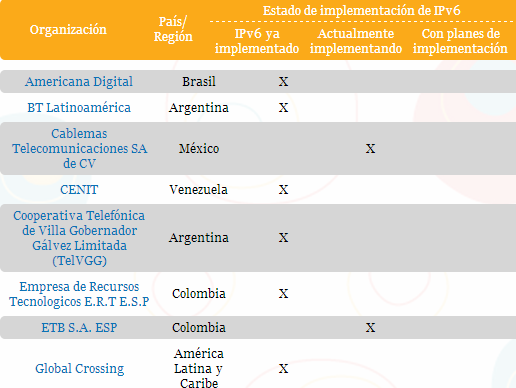
\includegraphics[height=1\textheight]{empresas ipv6 la.png}

\end{frame}

\end{document}
